\documentclass[conference]{IEEEtran}
\IEEEoverridecommandlockouts
\usepackage{cite}
\usepackage{xcolor}
\usepackage{mathtools}
\usepackage{footnote}
\usepackage{cancel}
\usepackage{xfrac}
\usepackage{amsmath,amssymb,amsfonts,amsthm}
\usepackage{algorithm}
\usepackage{algorithmicx}
\usepackage{algpseudocode}
\usepackage[hidelinks]{hyperref}
\usepackage{siunitx}
\usepackage{graphicx}
\usepackage{float}
\usepackage{tikz}
\usepackage{textcomp}
\usepackage[utf8]{inputenc}
\usepackage[english]{babel}

\usetikzlibrary{automata, positioning, arrows}
\newtheorem{theorem}{Theorem}

\def\BibTeX{{\rm B\kern-.05em{\sc i\kern-.025em b}\kern-.08em
    T\kern-.1667em\lower.7ex\hbox{E}\kern-.125emX}}

\hypersetup{colorlinks=false}

\begin{document}

\title{Segregation without Computation}

\author{
  \IEEEauthorblockN{Peter Mitrano\IEEEauthorrefmark{1} , Jordan Burkland\IEEEauthorrefmark{1}, Michael Giancola\IEEEauthorrefmark{1}, Carlo Pinciroli\IEEEauthorrefmark{1}}
  \IEEEauthorblockA{\IEEEauthorrefmark{1}Worcester Polytechnic Institute, Worcester, Massachusetts}
}

\maketitle

\section{Controller Analysis}

  We found from grid search that the parameters [$1$, $-0.6667$, $0.3333$, $1.0$, $1.0$, $0.0$] best achieve segregation as defined by our cluster metric cost function. The actual wheel speeds, which are scaled by $0.2$ to convert to \SI{}{\meter\per\second} are therefore [$0.2$, $-0.1333$, $0.06667$, $0.2$, $0.2$, $0.0$]. Now that we have found parameters that achieve what we consider segregation, we define the conditions under segregation is guaranteed. We first define the conditions under which aggregation between two isolated kin robots is guaranteed. Then we show that kin will aggregate with a static ring of kin. Finally, we show that non-kin will aggregate faster to kin than non-kin. All together, this explains much of the emergent behavior. More generally it demonstrates that we can prove useful things about complex emergent swarm behavior of these simple robots and controllers. In all of these proofs we will consider the controller found via grid search since it is the best controller. We also assume the controllers are in sync, that each motion is execute for the same $\Delta t$ at the same point in time, and that the robot has a fixed positive inter wheel distance $W$ and radius $r$.

    \begin{figure}[t!]
      \centering
      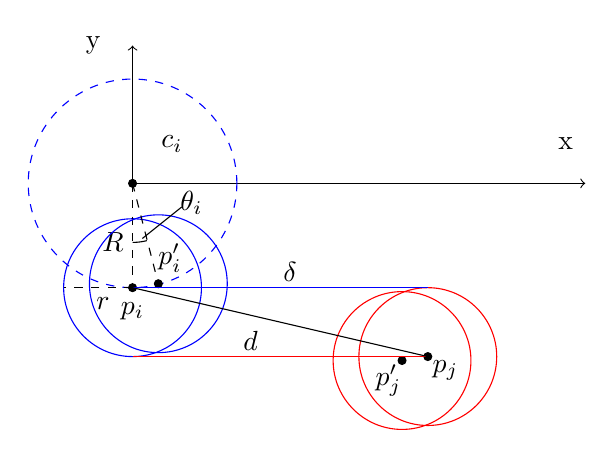
\begin{tikzpicture}[scale=25.0]
        \draw[->] (0,0) -- (0.23,0);
        \node at (0.22,.02) {x};
        \draw[->] (0,0) -- (0,0.07);
        \node at (-.02,0.07) {y};

         % c_i
        \filldraw (0,0) circle (.002);
        \node at (.02,.02) {$c_i$};
        \draw[blue, dashed] (0,0) circle (0.053);

         % p_i
        \filldraw (0,-0.053) circle (.002);
        \node at (0,-0.065) {$p_i$};
        \draw[blue] (0,-.053) circle (0.035);
        \node at (-0.01,-.03) {$R$};
        \draw[dashed] (0,0) -- (0,-0.053);
        \draw[dashed] (0,-0.053) -- (-0.035,-0.053);
        \node at (-0.015,-0.061) {$r$};

         % p'_i
        \filldraw (0.0131,-0.051) circle (.002);
        \node at (0.019,-0.038) {$p'_i$};
        \draw[blue] (0.0131,-0.051) circle (0.035);
        \draw[dashed] (0,0) -- (0.0131,-0.051);

         % p_j
        \filldraw (0.15, -0.088) circle (.002);
        \node at (0.159, -0.095) {$p_j$};
        \draw[red] (0.15, -0.088) circle (0.035);

         % p'_j
        \filldraw (0.1369, -0.09) circle (.002);
        \node at (0.13, -0.1) {$p'_j$};
        \draw[red] (0.1369, -0.09) circle (0.035);

        % delta
        \draw[blue] (0,-.053) -- (.15,-.053);
        \draw[red] (0,-.088) -- (.15,-.088);
        \node at (0.08, -0.045) {$\delta$};

        % theta
        \draw (0,-.03) arc [radius=.03, start angle=-90, end angle=-76];
        % TODO add theta annotation back
        \node at (.03,-.01) {$\theta_i$};
        \draw (.025,-.012) -- (.005, -.028);

        % d
        \draw (0,-0.053) -- (0.15, -0.088);
        \node at (0.06,-0.08) {$d$};
      \end{tikzpicture}
      \caption{The configuration of a robot aggregating to another kin where both robots see each other. $R$ is the radius of the robots path around the ICC.}
      \label{fig:kin_aggregation}
    \end{figure}

  \subsection{Aggregation of Two Kin}

    \begin{figure}[t!]
      \centering
			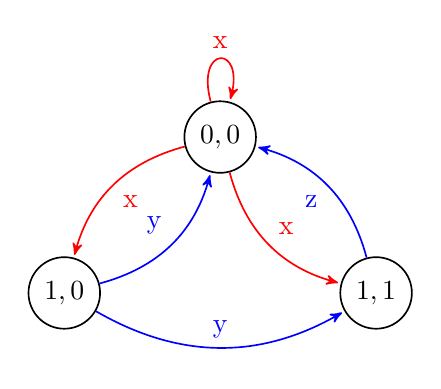
\begin{tikzpicture}[->,>=stealth',shorten >=1pt,auto,node distance=2.8cm, semithick]
				\node[state] (A)                    {$0,0$};
				\node[state] (B) [below left of=A]  {$1,0$};
				\node[state] (C) [below right of=A] {$1,1$};
        \node at (0, -2.5) (hidden) {};

				\path (A) edge [red, loop above] node {x} (A)
                  edge [red, bend right] node {x} (B)
                  edge [red, bend right] node {x} (C)
              (B) edge [blue, bend right] node {y} (C)
                  edge [blue, bend right] node {y} (A)
              (C) edge [blue, bend right] node {z} (A);
			\end{tikzpicture}
      \label{fig:fsm}
      \caption{State machine representation for two kin aggregation. (1,0) means robot $i$ has sensor state $I=0$, and robot $j$ has $I=1$. Blue arrows indicate transitions where the robots aggregate, and red indicates they may not aggregate. Letters indicate identical transitions. One can see visually in Figure \ref{fig:kin_aggregation} that impossible to transition from $(1,1)$ to $(1,0)$ because both robots rotate away from each other.}
		\end{figure}

    The set of all possible initial configurations of two robots $i$ and $j$ can be split into three possible states. Either neither robot sees the other $(0,0)$, one robot sees the other $(1,0)$, or both robots see each other $(1,1)$. In order to show that aggregation is guaranteed in all scenarios, we consider how these states evolve as a finite state machine (Figure \ref{fig:fsm}). For each sensor state $I=0,1,2$ there is a corresponding radius of rotation around the ICC which we call $R_0$, $R_1$, $R_2$ respectively. For each sensor state, There are three unique transitions between states in this state machine, which are called $x$, $y$ and $z$. For example, from state $(0,0)$ both robots will drive with speeds $v_{0_l}=0.2,v_{0_r}=-0.1333$, and as a result either the robots will continue to see nothing and transition back to $(0,0)$ or it could transition to the other two states.

    We show that the distance by which the robots aggregate during the blue transitions $y$ or $z$ is always greater than the distance they could possibly separate in any sequence of $x$ transitions. In other words, if we started at $(0,0)$, we can continue to loop there but when we eventually transition to another state, and the again transition out of that state (now along a blue arrow), we prove that the robots must be closer at then end then when they started.

    Intuitively, if the robots execute $(0,0)$ repeatedly they simply spin in a small circle, and so they're dispersion is bounded. The upper bound on how much the robots disperse in transition $x$ we call $s$, and it is equal to twice the radius of the curvature of the robots path $R_0$. Equation \eqref{eq:s_bound} formally defines $s$.

    \begin{equation} \label{eq:s_bound}
      \begin{split}
        s &= 2R_0 = 2\frac{W}{2}\bigg(\frac{v_{l_1} + v_{r_1}}{v_{l_1} - v_{r_1}}\bigg) = \frac{W}{4}\bigg(\frac{0.2 + -0.133}{0.2 - (-1.333)}\bigg) \\
        &= 0.8W
      \end{split}
    \end{equation}

    We need to show that, in transitions $y$ and $z$, the kin robots always aggregate more than $s$. We first demonstrate that the magnitude of aggregation, which can be described as $d'-d$ in Figure \ref{fig:kin_aggregation}, always decreases as the sensor ray length $\delta$ decreases. In other words, the closer the robots are, the less by which they aggregate. The conditions under which this is true are derived in Theorem \ref{thm:decrease}. From this we know that if the robots aggregate by more than $s$ at the smallest $\delta$, then they must also aggregate for all larger $\delta$. This second condition is derived in Theorem \ref{thm:one_see_cond} and \ref{thm:both_see_cond}, and the final conditions are shown below. We know the lower bound of $\delta$ is $\sqrt{2}r$ because this is the point at which the two robots of radius $r$ are touching.

    \begin{equation} \label{eq:two_kin_cond_1}
        \frac{1}{-W-r+W\cos(\theta_i)} \leq \sqrt{2}
    \end{equation}

    % TODO: maybe mention this second constrain is always true if the third one is
    \begin{equation} \label{eq:two_kin_cond_2}
      \begin{split}
        &\sqrt{(\sqrt{2}r_j - W\sin(\theta_i))^2 + (-W-r_j+W\cos(\theta_i))^2} \\
        & - \sqrt{3}r_j < \frac{\Delta t}{15W} + 1.6W\sin\bigg(\frac{\Delta t}{6W}\bigg)
      \end{split}
    \end{equation}

    \begin{equation} \label{eq:two_kin_cond_3}
      \begin{split}
        &\sqrt{(\sqrt{2}r_j - 2W\sin(\theta_i))^2 + (-r_j-2W+2W\cos(\theta_i))^2} \\
        & - \sqrt{3}r_j < \frac{\Delta t}{15W}
      \end{split}
    \end{equation}

    Ultimately, if Equations \eqref{eq:two_kin_cond_1}, \eqref{eq:two_kin_cond_2}, and \eqref{eq:two_kin_cond_3} are satisfied, we can say that from any initial configuration, two kin robots will eventually aggregate in a sort of two-steps-forward one-step-back fashion. This behavior is clearly demonstrated in our simulation and real robot experiments.

  \subsection{Aggregation with Ring of Kin}

    In this scenario, imagine an isolated kin robot which has sensed a ring of kin. Imagine the ring of kin as robot $j$ but with a different (larger) radius than the isolated robot $i$. If we consider the center of the ring static, we can define the conditions under which robot $i$ is guaranteed to be closer to the center of the ring. Robot $i$ starts at $p_i$ with sensor reading $I=1$. It then executes $v_{l_1} = 0.06667$ and $v_{r_1} = 0.2$ and arcs with radius $R_1$ to the left and ends up at position $p'_i$. We show that for a small $\Delta t$ that the robot moves closer to the center of the ring at $p_j$.

    The condition we need to satisfy is shown in Equation \eqref{eq:ring_agg}. The variable $r_j$ how denotes the radius of this ring, whereas $r$ still refers to the radius of a single robot.

    \begin{equation} \label{eq:ring_agg}
      \lVert p'_i - p_j \rVert < \lVert p_i - p_j \rVert
    \end{equation}

    We can expand Equation \eqref{eq:ring_agg} and derive a simple condition which describes for which values of $r$, $r_j$, $W$, $\Delta t$, this holds true for all $\delta$. The full derivation can be found in Theorem \ref{thm:aggregation_with_ring_of_kin}, and the result is shown in Equation \eqref{eq:ring_agg_result}.

    \begin{equation} \label{eq:ring_agg_result}
      \begin{split}
        &\sqrt{(\sqrt{2}r_j - 2W\sin(\theta_i))^2 + (-r_j-2W+2W\cos(\theta_i))^2} \\
        &-\sqrt{3}r_j < 0
      \end{split}
    \end{equation}

    Ultimately, we can use these geometric proof to make a useful assertions about the behavior of an individual in our swarm and of the swarm as a whole. While we have not shown that segregation is guaranteed in all cases, this may serve as a building block for more general claims.

  \subsection{Segregation}

    So far all of the behaviors we have discussed are actually just aggregation behaviors. Here we partially explain why segregation occurs by showing that between two robots $i$ and $j$, the kin robots aggregate faster than the non-kin robots. First, we need to explain why non-kin robots do in fact aggregate at all. It is counter intuitive that the optimal contorller for segregation aggregates non-kin. The key is that they aggregate more slowly, so only in absense of kin do non-kin aggregate. In our supplementary videos we include an example of an environment with only non-kin to demonstrate this.

    The conditions for non-kin aggregating follows the same steps as the proof for kin aggregating, except with different coordinates for $p_i$, $p_j$, and $p'_i$. The derivation is shown in Theorem \ref{thm:decrease2} If the resulting conditions at met, then non-kin are guaranteed to aggregate to kin.

    Next, to show that non-kin aggregate more slowly than kin, we show that the displacement during their kin step (the arc left with speeds $0.01666, 0.2$) is greater than the displacement during their non-kin step (with speeds $0.2, 0.0$).

    \begin{theorem} \label{thm:seg}
      The distance moved in the kin step is always greater than the distance moved in the non-kin step.
    \end{theorem}
    \begin{proof}
      We compare the arc lengths derived from the wheels speeds.
      \begin{align*}
        \theta_1 R_1 &> \theta_2 R_2 \\
        \frac{2\cancel{\Delta t}}{15\cancel{W}} \cancel{W} &> \frac{\cancel{2}\cancel{\Delta t}}{10\cancel{W}} \frac{\cancel{W}}{\cancel{2}} \\
        \frac{2}{15} &> \frac{1}{10} \\
      \end{align*}
    \end{proof}

    Note that we don't show that the kin step actully gets closer to the other robot, so in theory the longer kin step could aggregate less than the shorter non-kin step, but this at least partially justifies why kin aggregate faster.

  \subsection{Application to Real Swarm Robots}

    The above conditions for not hold true for all scenarios (such as those with large $\Delta t$), but we show that they do hold true for many popular robots in Table \ref{table:robots}.

    \begin{savenotes}
    \begin{table}
      \centering
      \caption{Aggregation is guaranteed for many differential drive swarm robots.}
      \begin{tabular}{|c|c|c|c|} \hline
        Robot & $r$ (m) & $W$ (m) & maximum $r_j$ (m) \\ \hline
        foot-bot\footnote{\href{https://github.com/ilpincy/argos3/blob/master/src/plugins/robots/foot-bot/simulator/footbot_entity.cpp}{ARGoS file footbot\_entity.cpp}} &
            0.085 & 0.14 & 74.619 \\ \hline
        Khephera IV\footnote{Khephera IV User Manual, page 66.} &
            0.07 & 0.1054 & 34.725 \\ \hline
        E-Puck 2\footnote{\href{http://projects.gctronic.com/epuck2/e-puck2-flyer.pdf}{http://projects.gctronic.com/epuck2/e-puck2-flyer.pdf}} &
            0.035 & 0.053 & 4.288 \\ \hline
        Kilobot\footnote{\href{https://www.k-team.com/mobile-robotics-products/kilobot/specifications}{https://www.k-team.com/mobile-robotics-products/kilobot/specifications}} &
            0.0165 & 0.030\footnote{only approximate} & 0.594 \\ \hline
      \end{tabular}
      \label{table:robots}
    \end{table}
    \end{savenotes}

\section{Experimental Results}

  \subsection{Evaluating the centroid-of-centroids cost function} \label{section:evaluting_cost_functions}

    When we implemented the centroid-of-centroids style cost function, we quickly found examples of configurations which were ranked undesirably. One example is shown below in Figure \ref{fig:cost_function_fuckup}. The behavior that looks like aggregation was given lower cost of $-8\cdot 10^{9}$, versus the behavior that looks like segregation was given a cost of $-5\cdot 10^{9}$.

    \begin{figure}[H]
      \centering
      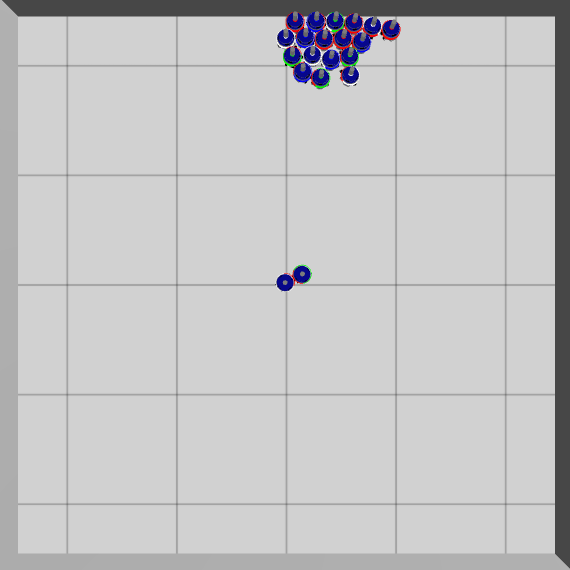
\includegraphics[width=0.49\linewidth]{./images/individual_0_gen_0.png}
      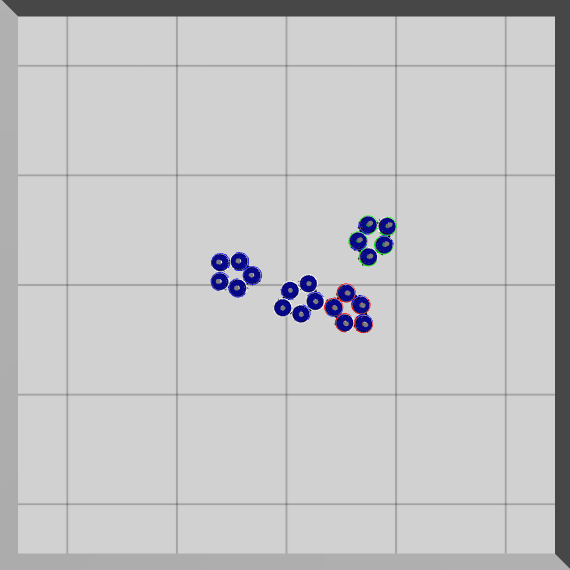
\includegraphics[width=0.49\linewidth]{./images/individual_0_gen_1_better.png}
      \caption{The left picture was given lower cost than the right, which is not desirable.}
      \label{fig:cost_function_fuckup}
    \end{figure}

  \subsection{Scalability Study} \label{section:scalability}

    In this experiment we investigate how segregation behavior scales with the number of classes and number of robots in the environment. We varied the number of classes from 1 to 25 and ran 100 trials of robots uniformly randomly distributed.

    \paragraph{Fixed number of robots per class}

    Because our cost function is independent of the number of classes, we first considered having 10 robots for each class. However, this also means that in the trial with 25 classes there are 25 times the total number of robots than in the 1-class trial. This means that occlusion of robots is more likely and so the cost increases with more classes. The results of this are plotted in Figure  \ref{fig:num_classes_10}.

    \paragraph{Fixed total number of robots}

    Another scenario is to consider a fixed number of robots and split them into more and more classes. We choose 100 robots because we are still able to get 4 robots per class at 25 classes. As you can see in Figure \ref{fig:num_classes_100}, the cost no longer increases as the number of classes increases. However, the cost for just a few classes is much higher. This is expected, because when there are many robots of a single class, our controller forms very large sparse rings where robots are too far apart to be considered clustered.

    Ultimately, we can say that our controller scales well to many classes with few robots, but not well to many robots of the same class.

    \begin{figure}[H]
      \centering
      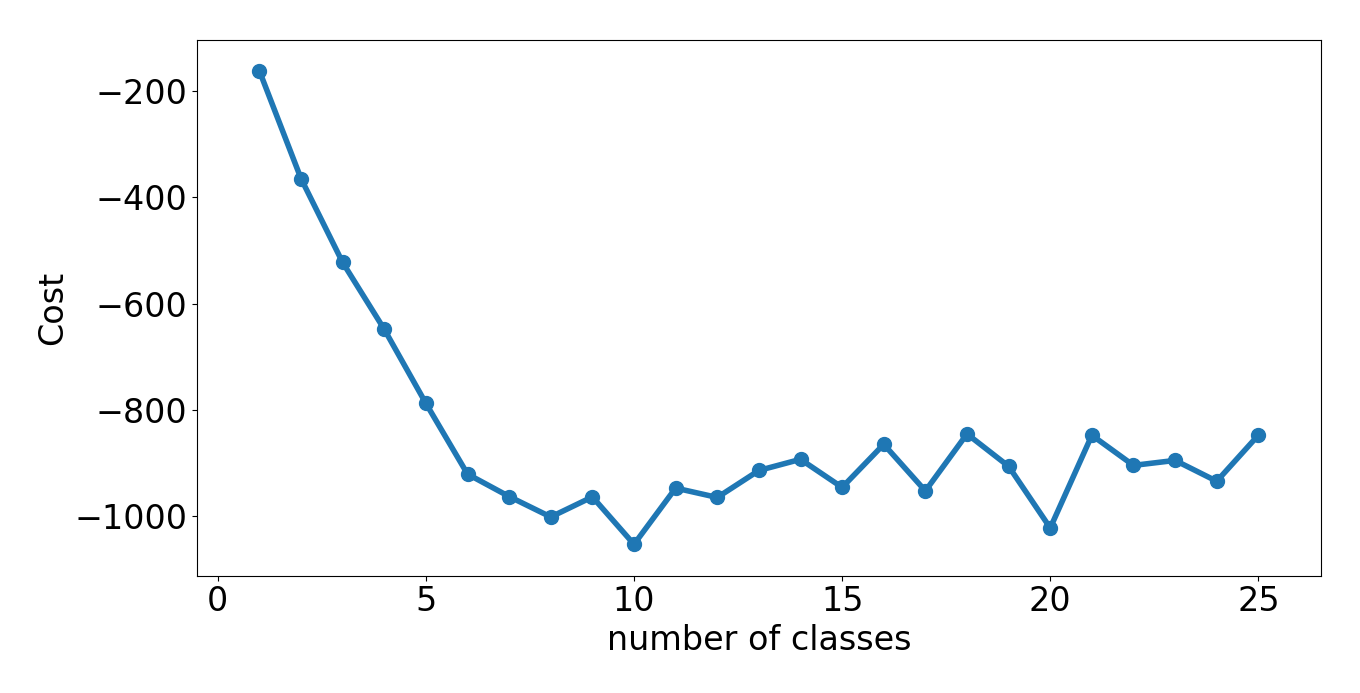
\includegraphics[width=1\linewidth]{./images/num_classes_vs_cost_100_robots.png}
      \caption{The average cost with 100 robots divided into N classes. More classes are lower cost partially because kin robots stay close enough to be considered clusters.}
      \label{fig:num_classes_100}
    \end{figure}

    \begin{figure}[H]
      \centering
      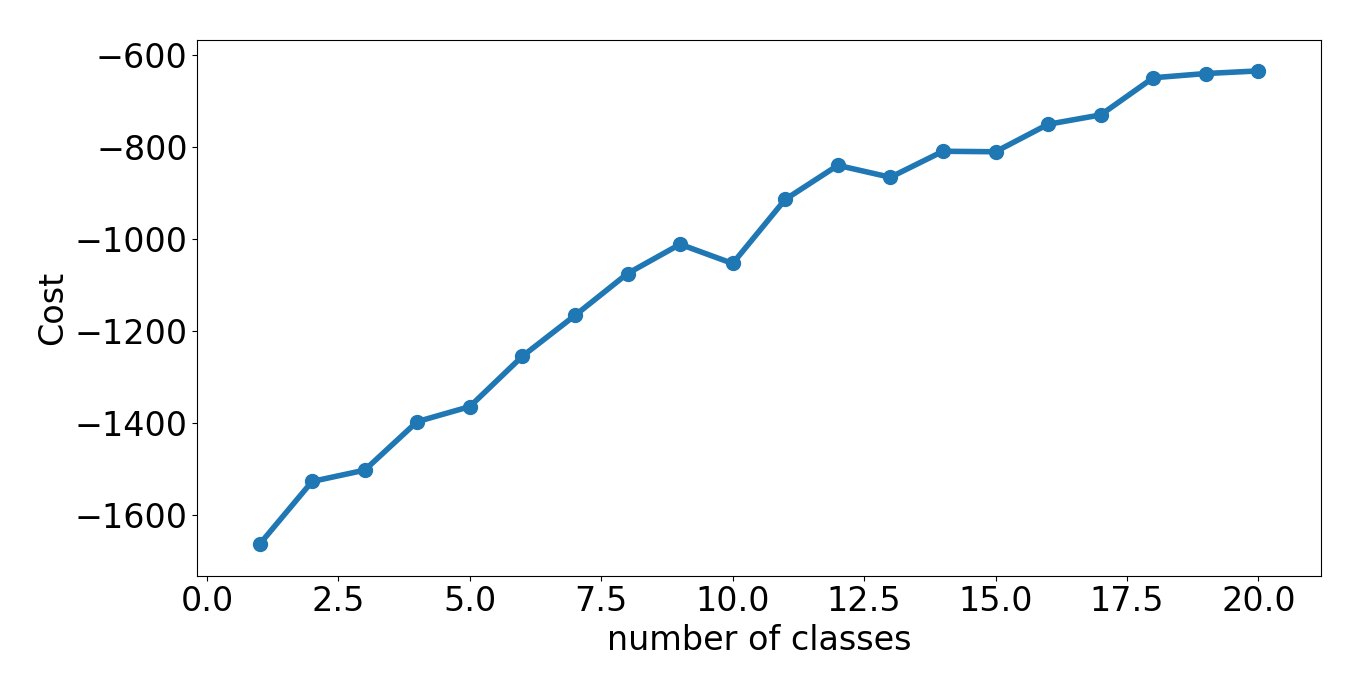
\includegraphics[width=1\linewidth]{./images/num_classes_vs_cost_10_per_class.png}
      \caption{The average cost with N classes, 10 robots per class. More classes are higher cost because other robots obstruct your view making it difficult to find kin.}
      \label{fig:num_classes_10}
    \end{figure}

  \subsection{The Effect of Implementation Details of the sensor} \label{section:sensor_impl}

    We found in our experiments that the implementation details of the line-of-sight sensor have a significant effect on the behavior of the controller.

    Initially, our method for determining sensor state from our simulated range-and-bearing sensors was to consider all the robots within some small angle in front of the robot and pick the closest one. This is very similar to what would be provided by a real-world camera that uses colored skirts on each robot and picks the largest blob as the robot to be detected. This sensor implementation works well and was used in all our genetic algorithm and grid search experiments. However, we found later that if the robots instead always prefer to react to kin over non-kin, you can form larger rings more quickly and robustly. For example, if there are two robots within the field of view of your sensor and the non-kin robot is closer, you will ignore it and execute the $I=1$ state which will drive you towards the farther away kin robot. Exploring exactly which of these implementation details have what effect on cost is left for future work.

  \subsection{The Effect of the Beam Angle} \label{section:beam_angle}

    On a real robot, there must be some finite beam angle to the theoretically line-of-sight sensor. We ran 100 trials in simulation with uniformly random initial distributions of 40 robots with various half beam angles. Figure \ref{fig:beam_angle} shows the results, as well as a diagram showing how we define half beam angle. The best half beam angle we tested was \ang{15}, and angles smaller or larger became progressively worse. We found that at lower beam angles, it was possible for a robot to become stuck in groups of two or three where the robots spent all their time looking at each other and not peeking around them to find kin. At larger angles, we believe the behavior fails because larger beam angles cause the rings to enlarge faster, which in turn causes the rings to be so large that they are not considered a cluster anymore and so the cost rises.

    \begin{figure}[H]
      \centering
      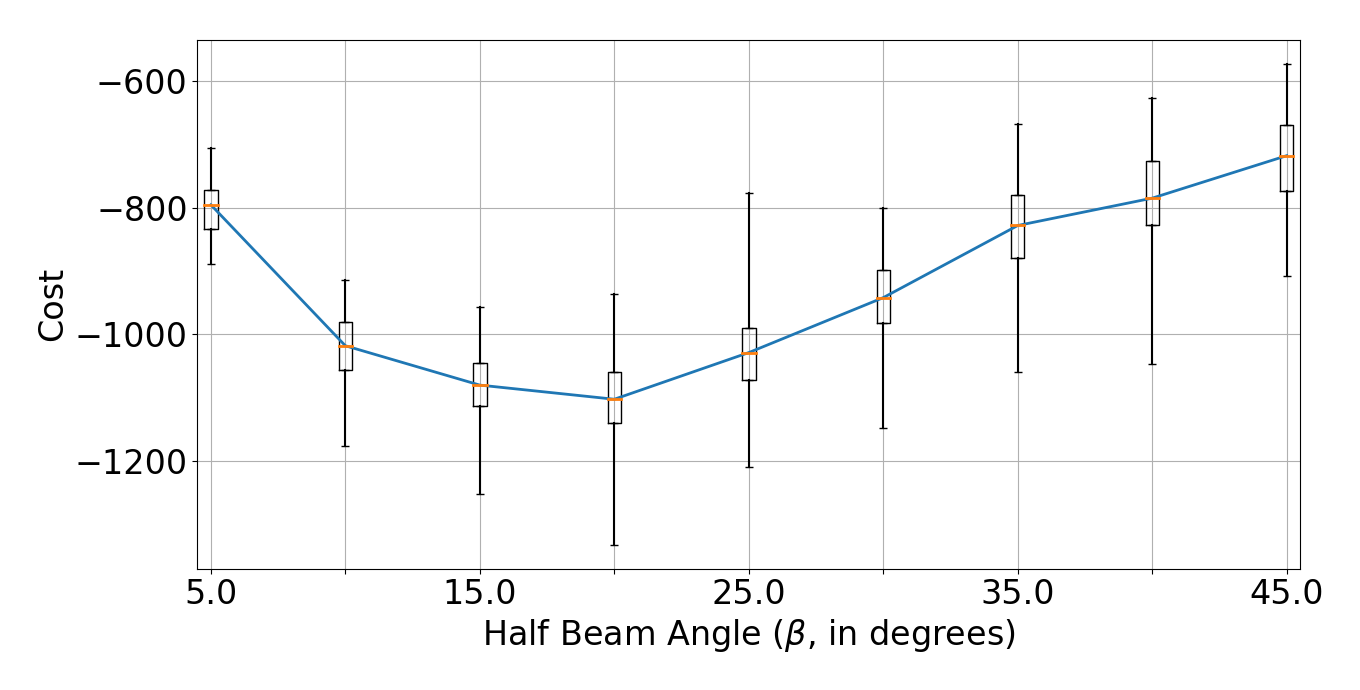
\includegraphics[width=1\linewidth]{./images/beam_angle.png}
      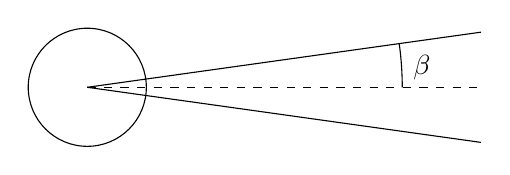
\begin{tikzpicture}
        \draw (0,0) circle (0.75);
        \draw (0,0) -- (5,0.7);
        \draw[dashed] (0,0) -- (5,0);
        \draw (0,0) -- (5,-0.7);
        \draw (4,0) arc [radius=4, start angle=0, end angle=8];
        \node at (4.25,0.25) {$\beta$};
      \end{tikzpicture}
      \caption{A \ang{15} degree half beam angle is best for segregation. Lower cost is better.}
      \label{fig:beam_angle}
    \end{figure}

  \subsection{The Effect of Beam Length} \label{section:beam_length}

    We also consider what happens if our theoretically infinite sensor now has finite range. We use \ang{15} half beam angle and the same experimental setup as with the beam angle experiments. Analogously to \cite{gauci_self-organized_2014}, we consider the maximum range of the sensor as the diagonal length of the square in which the robot are initially distributed. In all our experiments, this box was \SI{5}{\meter\square}, so we consider a range of \SI{7.07}{\meter} to be effectively unlimited. We report the costs for beam lengths as a fraction of this maximum range. As shown in Figure \ref{fig:beam_length}, a beam length of 35\% of the theoretical maximum performs just as well. Below this, the performance degrades. However, even a beam length of 7\% of unlimited is more effective than zero length at segregation. In our experiment watching many simulations, beam length should also be scaled with the total number of robots as well as the initial distance between robots. When the beam length is short, there are many cases where two rings of kin robots form at different points in the environment, and in order for these two rings to join the robots must have sufficiently long beam length in order to detect each other.

    \begin{figure}
      \centering
      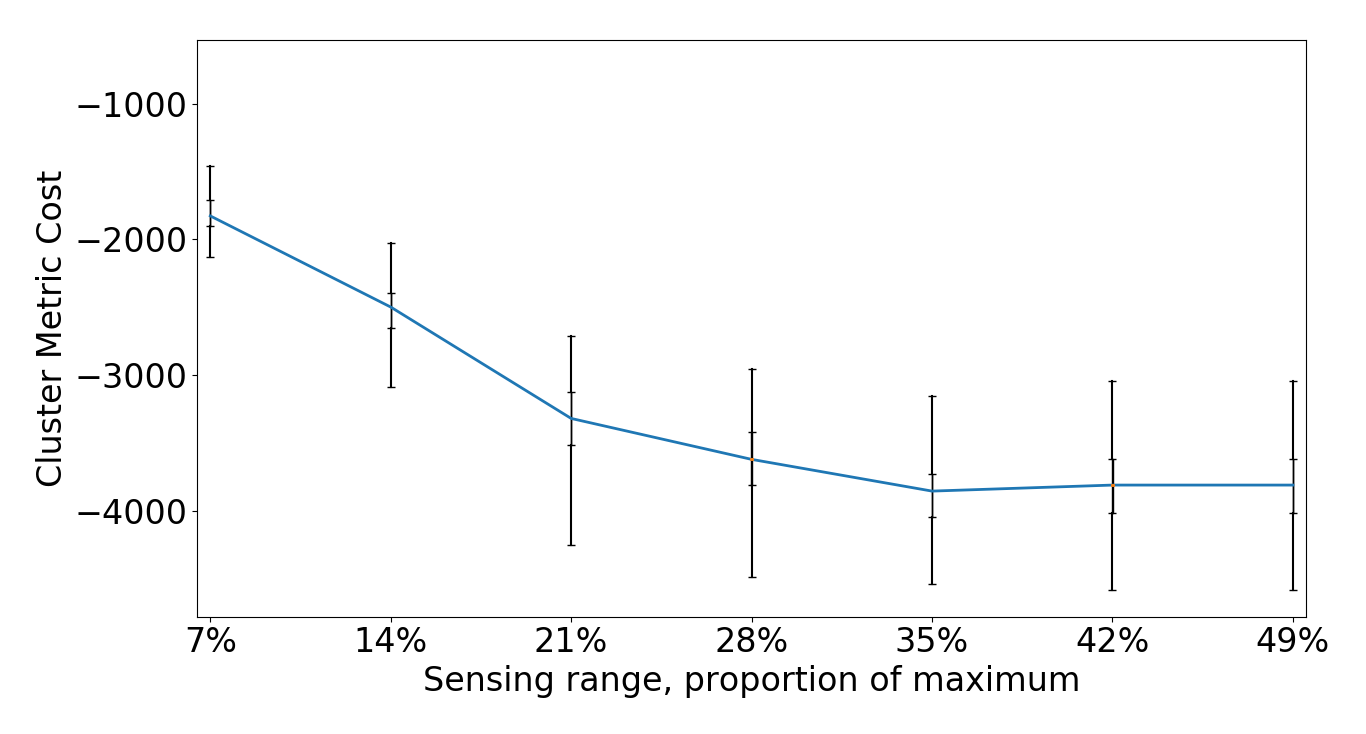
\includegraphics[width=1\linewidth]{./images/beam_length.png}
      \caption{Segregation is robust to very finite sensor beam lengths. The blue bar indicates the worst (highest) attainable cost in which all robots are isolated from any kin.}
      \label{fig:beam_length}
    \end{figure}

\section{Conclusion}

  In this paper, we demonstrate that memoryless, computeless robots are capable of $n$-class segregation. We use a simple controller design consisting of a 6-tuple. This controller is invariant to the number of classes, so any given controller can work for any number of classes. To quickly find a quality controller, we evolved one using a basic genetic algorithm, but we also performed a grid search to make claims about the full parameter space. We investigated the effect of sensor implementation details and the number of robots and classes on performance. We find that robust segregation is possible, although not guaranteed. Instead, we prove that aggregation of kin robots is guaranteed when reasonable conditions on controller frequency and inner wheel distance are met.

\bibliography{RBE595.bib}
\bibliographystyle{unsrt}

\onecolumn
\appendix
\section{Appendix}

    \begin{align}
      \begin{split} \label{eq:theta_and_r}
        \theta_i &= \Delta t\omega = \Delta t \frac{v_{r_1} - v_{l_1}}{W} = \Delta t \frac{0.2 - 0.06667}{W} = \frac{2\Delta t}{15W} \\
        R_1 &= \frac{W}{2}\bigg(\frac{v_{r_1} + v_{l_1}}{v_{r_1} - v_{l_1}}\bigg) = \frac{W}{2}\bigg(\frac{0.2 + 0.06667}{0.2 - 0.06667}\bigg) = W
      \end{split}
    \end{align}

    From Figure \ref{fig:kin_aggregation} we can define the coordinates of $p_i$, $p_j$, $p'_i$, and $p'_j$.

    \begin{equation} \label{eq:two_kin_vars_1}
      \begin{split}
        p_i = \begin{bmatrix}0 \\ -R_1\end{bmatrix} \\
        p_j = \begin{bmatrix}\delta \\ -(R_1+r_j)\end{bmatrix} \\
        p'_i = \begin{bmatrix}R_1\sin(\theta_i) \\ -R_1\cos(\theta_i)\end{bmatrix} \\
        p'_j = \begin{bmatrix}\delta - R_1\sin(\theta_i) \\ -(R_1+r) - (R_1-R_1\cos(\theta_i))\end{bmatrix} \\
      \end{split}
    \end{equation}

  \begin{theorem} \label{thm:decrease}
    Robots aggregate by less the closer they are
  \end{theorem}
  \begin{proof}

    We show that $d'-d$ always decreases as $\delta$ decreases (until its minimum of $\sqrt{2}r$). This is true if the derivative $\frac{\partial}{\partial\delta}(d'-d) \leq 0$, $\forall \delta>\sqrt{2}r$.

    \begin{align*}
      \frac{\partial}{\partial\delta}(d'-d) &< 0 \\
      \frac{\partial}{\partial\delta}\big(\lVert p_j - p'_i \rVert - \lVert p_j - p_i \rVert\big) &\leq 0 \\
      \frac{\partial}{\partial\delta}\bigg(\sqrt{(p_{j_x} - p'_{i_x})^2 + (p_{j_y} - p'_{i_y})^2} - \sqrt{(p_{j_x} - p_{i_x})^2 + (p_{j_y} - p_{i_y})^2}\bigg) &\leq 0 \\
      \frac{\partial}{\partial\delta}\bigg(\sqrt{(\delta - b)^2 + a} - \sqrt{(\delta- 0)^2 + (p_{j_y} - p_{i_y})^2}\bigg) &\leq 0 \\
      \frac{\partial}{\partial\delta}\bigg(\sqrt{(\delta - b)^2 + a} - \sqrt{\delta^2 + (p_{j_y} - p_{i_y})^2}\bigg) &\leq 0 \\
      \frac{\partial}{\partial\delta}\bigg(\sqrt{(\delta-b)^2 + a} - \sqrt{\delta^2 + (-(R_1+r) - R_1)^2}\bigg) &\leq 0 \\
      \frac{\partial}{\partial\delta}\bigg(\sqrt{(\delta-b)^2 + a} - \sqrt{\delta^2 + r^2}\bigg) &\leq 0 \\
      \frac{1}{2}\Big[((\delta-b)^2 + a)^{-\frac{1}{2}}(2\delta-2b) - (\delta^2 + r^2)^{-\frac{1}{2}}(2\delta)\Big] &\leq 0 \\
      ((\delta-b)^2 + a)^{-\frac{1}{2}}(\delta-b) - (\delta^2 + r^2)^{-\frac{1}{2}}(\delta) &\leq 0 \\
      ((\delta-b)^2 + a)^{-\frac{1}{2}}(\delta-b) &\leq (\delta^2 + r^2)^{-\frac{1}{2}}(\delta) \\
      (\delta^2 + r^2)^{\frac{1}{2}}(\delta-b) &\leq (\delta)((\delta-b)^2 + a)^{\frac{1}{2}} && \text{all terms are positive, see Theorem \ref{thm:d-b}} \\
      (\delta^2 + r^2)(\delta-b)^2 &\leq (\delta)^2((\delta-b)^2 + a) && \text{squaring preserves inequality for positive terms} \\
      \cancel{\delta^2(\delta-b)^2} + r^2(\delta-b)^2 &\leq \cancel{\delta^2(\delta-b)^2} + a\delta^2 \\
      r^2(\delta-b)^2 &\leq a\delta^2 \\
      r^2(\delta^2-2b\delta+b^2) &\leq a\delta^2 \\
      r^2\delta^2 - r^22b\delta + r^2b^2 &\leq a\delta^2 \\
      (r^2 - a)\delta^2 - r^22b\delta + r^2b^2 &\leq 0 && \text{If parabola opens down} \\
      \frac{\partial}{\partial\delta}\big((r^2 - a)\delta^2 - r^22b\delta + r^2b^2\big) &\leq 0 \\
      2(r^2 - a)\delta - r^22b &\leq 0 \\
      2(r^2 - a) &\leq 0 \\
      \text{where}\  a=(-R_1-r-R_1\cos(\theta_i)),&\  b=-R_1\cos(\theta_i)
    \end{align*}

    If $2(r^2 - a) \leq 0$ and $(r^2 - a)2r^2 - r^22b\sqrt{2}r + r^2b^2 \leq 0$, then the change in distance $d'-d$ strictly decreases as $\delta$ increases. In other words, the amount that the two robots get closer is smallest when they are as close as possible. Because of this property, we can guarantee aggregation by showing that $d'-d<s$ when $d$ is at its minimum of $\sqrt{2}r$. In other words, if these two simple analytic conditions are satisfied, than aggregation between two kin robots is guaranteed. For convenience, we show the expanded forms of $d'-d$ for the two possible cases. To apply this, substitute the parameters of your robot into the two equations below and see if the conditions hold true.

  \end{proof}

  \begin{theorem} \label{thm:one_see_cond}
    $d'-d<s$ in state $(1,0)$ when one robot sees the other.
  \end{theorem}
  \begin{proof}

    In this state, robot $i$ will arc left with speeds $0.06667, 0.2$ and robot $j$ will rotate right with speeds $0.2, -0.1333$. Robot $i$ advances towards $j$ along a slight arc, whereas $j$ rotates mostly in place. Because $j$ is not stationary, there is an additional amount which it could move away from $i$, so in addition to showing that $d'-d<s$ we must add another approximate value to $s$ which we'll call $s'$. This maximum distance $j$ can move in one time step is the length of the chord defined by the radius $R_0$ (radius of turn for sensor $I=0$) and angle $\theta_j$. Equation \eqref{eq:s'} shows the full definition of this bound.

    \begin{equation} \label{eq:s'}
      \begin{split}
        \theta_j &= \Delta t\omega = \Delta t \frac{v_{l_1} - v_{r_1}}{W} = \Delta t \frac{0.2 - (-0.1333)}{W} = \frac{\Delta t}{3W} \\
        s' &= 2R_0\sin\bigg(\frac{\theta_j}{2}\bigg) = 2(0.8W)\sin\bigg(\frac{\Delta t}{6W}\bigg) = 1.6W\sin\bigg(\frac{\Delta t}{6W}\bigg)
      \end{split}
    \end{equation}

    \begin{align*}
      d' - d &< s + s' \\ %TODO (peter) account for the other s' which is from robot J rotating
      \lVert p_j - p'_i \rVert - \lVert p_j - p_i \rVert &< s + s' \\
      \sqrt{(p_{j_x} - p'_{i_x})^2 + (p_{j_y} - p'_{i_y})^2} - \sqrt{(p_{j_x} - p_{i_x})^2 + (p_{j_y} - p_{i_y})^2} &< s + s' \\
      \sqrt{(\sqrt{2}r_j - R_1\sin(\theta_i))^2 + (-(R_1+r_j) - (-R_1\cos(\theta_i)))^2} - \sqrt{(\sqrt{2}r_j - 0)^2 + (-(R_1+r_j) - (-R_1))^2} &< s + s' \\
      \sqrt{(\sqrt{2}r_j - R_1\sin(\theta_i))^2 + (-R_1-r_j+R_1\cos(\theta_i))^2} - \sqrt{2r_j^2 + r_j^2} &< s + s' \\
      \sqrt{(\sqrt{2}r_j - W\sin(\theta_i))^2 + (-W-r_j+W\cos(\theta_i))^2} - \sqrt{3}r_j &< \frac{\Delta t}{15W} + 1.6W\sin\bigg(\frac{\Delta t}{6W}\bigg)
    \end{align*}

  \end{proof}

  \begin{theorem} \label{thm:both_see_cond}
    $d'-d<s$ in state $(1,1)$ when both robots see each other.
  \end{theorem}
  \begin{proof}

    \begin{align*}
      d' - d  &< s \\
      \lVert p'_j - p'_i \rVert - \lVert p_j - p_i \rVert &< s \\
      \sqrt{(p'_{j_x} - p'_{i_x})^2 + (p'_{j_y} - p'_{i_y})^2} - \sqrt{(p_{j_x} - p_{i_x})^2 + (p_{j_y} - p_{i_y})^2} &< s \\
      \sqrt{((\sqrt{2}r_j - 2R_1\sin(\theta_i))^2 + ((-(R_1+r_j) - (R_1-R_1\cos(\theta_i))) - (-R_1\cos(\theta_i)))^2} - \sqrt{2r_j^2 + (-(R_1+r_j) - (-R_1))^2} &< s \\
      \sqrt{(\sqrt{2}r_j - 2R_1\sin(\theta_i))^2 + (-r_j-2R_1+2R_1\cos(\theta_i))^2} - \sqrt{2r_j^2 + r_j^2} &< s \\
      \sqrt{(\sqrt{2}r_j - 2W\sin(\theta_i))^2 + (-r_j-2W+2W\cos(\theta_i))^2} - \sqrt{3}r_j &< \frac{\Delta t}{15W}
    \end{align*}

  \end{proof}

  \begin{theorem}\label{thm:d-b}
    Proof that $(\delta-b)>0$
  \end{theorem}
  \begin{proof}
    \begin{align*}
      \delta - b &> 0 \\
      \delta - W\sin(\theta_i) &> 0 \\
      \sqrt{2}r - W\sin(\theta_i) &> 0 && \text{lower bound of }\delta \\
      \sqrt{2}r - W\sin(\theta_i) &> 0 && \text{The robot must be wider than its track width, } r \geq \tfrac{W}{2} \\
      \tfrac{\sqrt{2}}{2}W - W\sin(\theta_i) &> 0 \\
      \tfrac{\sqrt{2}}{2} - \sin(\theta_i) &> 0 \\
      \tfrac{\sqrt{2}}{2} &> \sin(\theta_i) \\
      \tfrac{\pi}{4} &> \theta_i \\
    \end{align*}
  \end{proof}

  \pagebreak

  \begin{theorem} \label{thm:aggregation_with_ring_of_kin}
    An isolated kin robot will aggregate to a ring of kin.
  \end{theorem}
  \begin{proof}
  \end{proof}

  \pagebreak


  \begin{theorem} \label{thm:decrease2}
    Robots aggregate by less the closer they are, in the non-kin case.
  \end{theorem}
  \begin{proof}

    We show that $d'-d$ always decreases as $\delta$ decreases (until its minimum of $\sqrt{2}r$). This is true if the derivative $\frac{\partial}{\partial\delta}(d'-d) \leq 0$, $\forall \delta>\sqrt{2}r$.

    \begin{align*}
      \frac{\partial}{\partial\delta}(d'-d) &< 0 \\
      \frac{\partial}{\partial\delta}\big(\lVert p_j - p'_i \rVert - \lVert p_j - p_i \rVert\big) &\leq 0 \\
      \frac{\partial}{\partial\delta}\bigg(\sqrt{(p_{j_x} - p'_{i_x})^2 + (p_{j_y} - p'_{i_y})^2} - \sqrt{(p_{j_x} - p_{i_x})^2 + (p_{j_y} - p_{i_y})^2}\bigg) &\leq 0 \\
      \frac{\partial}{\partial\delta}\bigg(\sqrt{(\delta - b)^2 + a} - \sqrt{(\delta - 0)^2 + (p_{j_y} - p_{i_y})^2}\bigg) &\leq 0 \\
      \frac{\partial}{\partial\delta}\bigg(\sqrt{(\delta - b)^2 + a} - \sqrt{\delta^2 + (p_{j_y} - p_{i_y})^2}\bigg) &\leq 0 \\
      \frac{\partial}{\partial\delta}\bigg(\sqrt{(\delta-b)^2 + a} - \sqrt{\delta^2 + (r-0)^2}\bigg) &\leq 0 \\
      \frac{\partial}{\partial\delta}\bigg(\sqrt{(\delta-b)^2 + a} - \sqrt{\delta^2 + r^2}\bigg) &\leq 0 \\
      \frac{1}{2}\Big[((\delta-b)^2 + a)^{-\frac{1}{2}}(2\delta-2b) - (\delta^2 + r^2)^{-\frac{1}{2}}(2\delta)\Big] &\leq 0 \\
      ((\delta-b)^2 + a)^{-\frac{1}{2}}(\delta-b) - (\delta^2 + r^2)^{-\frac{1}{2}}(\delta) &\leq 0 \\
      ((\delta-b)^2 + a)^{-\frac{1}{2}}(\delta-b) &\leq (\delta^2 + r^2)^{-\frac{1}{2}}(\delta) \\
      (\delta^2 + r^2)^{\frac{1}{2}}(\delta-b) &\leq (\delta)((\delta-b)^2 + a)^{\frac{1}{2}} && \text{all terms are positive, see Theorem \ref{thm:d-b}} \\
      (\delta^2 + r^2)(\delta-b)^2 &\leq (\delta)^2((\delta-b)^2 + a) && \text{squaring preserves inequality for positive terms} \\
      \cancel{\delta^2(\delta-b)^2} + r^2(\delta-b)^2 &\leq \cancel{\delta^2(\delta-b)^2} + a\delta^2 \\
      r^2(\delta-b)^2 &\leq a\delta^2 \\
      r^2(\delta^2-2b\delta+b^2) &\leq a\delta^2 \\
      r^2\delta^2 - r^22b\delta + r^2b^2 &\leq a\delta^2 \\
      (r^2 - a)\delta^2 - r^22b\delta + r^2b^2 &\leq 0 && \text{If parabola opens down} \\
      \frac{\partial}{\partial\delta}\big((r^2 - a)\delta^2 - r^22b\delta + r^2b^2\big) &\leq 0 \\
      2(r^2 - a)\delta - r^22b &\leq 0 \\
      2(r^2 - a) &\leq 0 \\
      \text{where}\  a=(-R_1-r-R_1\cos(\theta_i)),&\  b=-R_1\cos(\theta_i)
    \end{align*}

    If $2(r^2 - a) \leq 0$ and $(r^2 - a)2r^2 - r^22b\sqrt{2}r + r^2b^2 \leq 0$, then the change in distance $d'-d$ strictly decreases as $\delta$ increases.
  \end{proof}

\end{document}
